% Options for packages loaded elsewhere
\PassOptionsToPackage{unicode}{hyperref}
\PassOptionsToPackage{hyphens}{url}
%
\documentclass[
  english,
  man,floatsintext]{apa6}
\usepackage{lmodern}
\usepackage{amssymb,amsmath}
\usepackage{ifxetex,ifluatex}
\ifnum 0\ifxetex 1\fi\ifluatex 1\fi=0 % if pdftex
  \usepackage[T1]{fontenc}
  \usepackage[utf8]{inputenc}
  \usepackage{textcomp} % provide euro and other symbols
\else % if luatex or xetex
  \usepackage{unicode-math}
  \defaultfontfeatures{Scale=MatchLowercase}
  \defaultfontfeatures[\rmfamily]{Ligatures=TeX,Scale=1}
\fi
% Use upquote if available, for straight quotes in verbatim environments
\IfFileExists{upquote.sty}{\usepackage{upquote}}{}
\IfFileExists{microtype.sty}{% use microtype if available
  \usepackage[]{microtype}
  \UseMicrotypeSet[protrusion]{basicmath} % disable protrusion for tt fonts
}{}
\makeatletter
\@ifundefined{KOMAClassName}{% if non-KOMA class
  \IfFileExists{parskip.sty}{%
    \usepackage{parskip}
  }{% else
    \setlength{\parindent}{0pt}
    \setlength{\parskip}{6pt plus 2pt minus 1pt}}
}{% if KOMA class
  \KOMAoptions{parskip=half}}
\makeatother
\usepackage{xcolor}
\IfFileExists{xurl.sty}{\usepackage{xurl}}{} % add URL line breaks if available
\IfFileExists{bookmark.sty}{\usepackage{bookmark}}{\usepackage{hyperref}}
\hypersetup{
  pdftitle={English Negative Constructions and Communicative Functions in Early Child Language},
  pdfauthor={1 \& 2},
  pdflang={en-EN},
  pdfkeywords={negation; acquisition; development, semantics, pragmatics, syntax, child language.},
  hidelinks,
  pdfcreator={LaTeX via pandoc}}
\urlstyle{same} % disable monospaced font for URLs
\usepackage{graphicx,grffile}
\makeatletter
\def\maxwidth{\ifdim\Gin@nat@width>\linewidth\linewidth\else\Gin@nat@width\fi}
\def\maxheight{\ifdim\Gin@nat@height>\textheight\textheight\else\Gin@nat@height\fi}
\makeatother
% Scale images if necessary, so that they will not overflow the page
% margins by default, and it is still possible to overwrite the defaults
% using explicit options in \includegraphics[width, height, ...]{}
\setkeys{Gin}{width=\maxwidth,height=\maxheight,keepaspectratio}
% Set default figure placement to htbp
\makeatletter
\def\fps@figure{htbp}
\makeatother
\setlength{\emergencystretch}{3em} % prevent overfull lines
\providecommand{\tightlist}{%
  \setlength{\itemsep}{0pt}\setlength{\parskip}{0pt}}
\setcounter{secnumdepth}{-\maxdimen} % remove section numbering
% Make \paragraph and \subparagraph free-standing
\ifx\paragraph\undefined\else
  \let\oldparagraph\paragraph
  \renewcommand{\paragraph}[1]{\oldparagraph{#1}\mbox{}}
\fi
\ifx\subparagraph\undefined\else
  \let\oldsubparagraph\subparagraph
  \renewcommand{\subparagraph}[1]{\oldsubparagraph{#1}\mbox{}}
\fi
% Manuscript styling
\usepackage{upgreek}
\captionsetup{font=singlespacing,justification=justified}

% Table formatting
\usepackage{longtable}
\usepackage{lscape}
% \usepackage[counterclockwise]{rotating}   % Landscape page setup for large tables
\usepackage{multirow}		% Table styling
\usepackage{tabularx}		% Control Column width
\usepackage[flushleft]{threeparttable}	% Allows for three part tables with a specified notes section
\usepackage{threeparttablex}            % Lets threeparttable work with longtable

% Create new environments so endfloat can handle them
% \newenvironment{ltable}
%   {\begin{landscape}\begin{center}\begin{threeparttable}}
%   {\end{threeparttable}\end{center}\end{landscape}}
\newenvironment{lltable}{\begin{landscape}\begin{center}\begin{ThreePartTable}}{\end{ThreePartTable}\end{center}\end{landscape}}

% Enables adjusting longtable caption width to table width
% Solution found at http://golatex.de/longtable-mit-caption-so-breit-wie-die-tabelle-t15767.html
\makeatletter
\newcommand\LastLTentrywidth{1em}
\newlength\longtablewidth
\setlength{\longtablewidth}{1in}
\newcommand{\getlongtablewidth}{\begingroup \ifcsname LT@\roman{LT@tables}\endcsname \global\longtablewidth=0pt \renewcommand{\LT@entry}[2]{\global\advance\longtablewidth by ##2\relax\gdef\LastLTentrywidth{##2}}\@nameuse{LT@\roman{LT@tables}} \fi \endgroup}

% \setlength{\parindent}{0.5in}
% \setlength{\parskip}{0pt plus 0pt minus 0pt}

% \usepackage{etoolbox}
\makeatletter
\patchcmd{\HyOrg@maketitle}
  {\section{\normalfont\normalsize\abstractname}}
  {\section*{\normalfont\normalsize\abstractname}}
  {}{\typeout{Failed to patch abstract.}}
\patchcmd{\HyOrg@maketitle}
  {\section{\protect\normalfont{\@title}}}
  {\section*{\protect\normalfont{\@title}}}
  {}{\typeout{Failed to patch title.}}
\makeatother
\shorttitle{Negation and communicative functions}
\keywords{negation; acquisition; development, semantics, pragmatics, syntax, child language.\newline\indent Word count: X}
\usepackage{lineno}

\linenumbers
\usepackage{csquotes}
\ifxetex
  % Load polyglossia as late as possible: uses bidi with RTL langages (e.g. Hebrew, Arabic)
  \usepackage{polyglossia}
  \setmainlanguage[]{english}
\else
  \usepackage[shorthands=off,main=english]{babel}
\fi

\title{English Negative Constructions and Communicative Functions in Early Child Language}
\author{\textsuperscript{1} \& \textsuperscript{2}}
\date{}


\authornote{

Add complete departmental affiliations for each author here. Each new line herein must be indented, like this line.

Enter author note here.

Correspondence concerning this article should be addressed to , . E-mail:

}

\affiliation{\vspace{0.5cm}\textsuperscript{1} \\\textsuperscript{2} }

\abstract{
How does negation emerge in early conceptual and linguistic development? Previous research has hypothesized that negation develops to express different communicative functions such as rejection, non-existence, or prohibition. However, these functions pro been challenging to detect and classify by human annotators using contextual cues. Consequently, in previous research we pro been limited to relatively small number of children and small samples of their speech. In this study, we consider specific syntactic constructions as proxies for communicative functions and examine their developmental trajectories in children's speech. We used automatic annotation and identification of seven different functions in a large corpus of child-parent interactions. Our analyses demonstrated frequent usage of negation in all seven functions between the ages of 24 - 36 months; yet there are notable differences in production variability of negation depending on the specifc function examined.
}



\begin{document}
\maketitle

\hypertarget{introduction}{%
\section{Introduction}\label{introduction}}

Negation is an abstract concept crucial to everyday communication. It can help a coffee shop divide its menu into \enquote{coffee} and \enquote{not coffee} sections, with the \enquote{not coffee} section bringing together diverse items with no common label. It can inform us to regulate each others' actions in a sign like \enquote{no mask, no entry}. It can also communicate our deepest wants and dislikes as in \enquote{I don't like Mondays}. But how does the abstract concept of negation emerge in the human mind? What are the specific communicative functions that negation combines with in early language development?

Starting a century and a half ago, Darwin (1872) thought that negation has roots in the expression of human emotions and desires. He hypothesized the earliest manifestation of negation and affirmation in infants is when they refuse food from parents, by withdrawing their heads laterally, or when they accept the food, by inclining their heads forward. He suggested that head shaking and nodding as common gestures for negation and affirmation pro developed from this early habit. Similarly, many researchers studying early functions of negative morphemes like \emph{no} proposed that children use them to \enquote{reject} or \enquote{refuse} (Bloom, 1970; Choi, 1988; Pea, 1978). For example, when they are asked \enquote{do you want juice?}, they may say \enquote{no}, \enquote{not want it}, or \enquote{don't like it}. Pea (1978) proposed this negation function is the first to emerge in children's early speech.

Bloom (1970) argued that the use of negation to expresses \enquote{non-existence} emerges before rejection or refusal. For example, when an object that children expect to be present is not present, children may say: \enquote{no window}, \enquote{no fish in the bathroom}, or \enquote{I do not pro underpants}. Two close concepts to non-existence are \enquote{disappearance} and \enquote{non-occurrence} (Pea, 1978; Villiers \& Villiers, 1979). Disappearance refers to situations where an object disappears and children use negation to express it (e.g.~\enquote{no food. all gone} or \enquote{no more noise}). Non-occurrence refers to cases when an expected action or event does not occur as in \enquote{not working} or \enquote{doggie not barking}. Some researchers referred to these cases as \enquote{failures} and included examples like \enquote{no fit in da box} or \enquote{it don't fit} (Cameron-Faulkner, Lieven, \& Theakston, 2007; Choi, 1988). Non-existence can also be expressed by negation of locative prepositional phrases (e.g.~\enquote{no in there} or \enquote{daddy was not on the phone}). While rejection was hypothesized to interact with human emotions and desires, non-existence (broadly construed to include \enquote{disappearance} and \enquote{non-occurrence}) likely interacts with human perception. Choi (1988) proposed that children's early linguistic negation is used to express both rejection and non-existence.

Additionally, Choi (1988) introduced \enquote{prohibition} and suggested that it emerges as early as rejection and non-existence. In cases of prohibition, children use negation to stop others from performing actions; for example \enquote{don't go} or \enquote{do not spill milk}. A special case of prohibition is \enquote{self-prohibition}. For example, a child may approach prohibited food but immediately say \enquote{no, don't eat} to stop themselves. A function similar to prohibition is \enquote{inability} (e.g.~\emph{I can't reach} / \emph{I cannot zip it}), in that both involve conceptualizing actions and negating them, possibly interacting with early development of motor control. Choi (1988) suggested that expression of inability emerges after the first phase, namely non-existence, rejection, and prohibition.

\enquote{Denial} is another function of negation that is argued to be late in development. Bloom (1970) defined it as asserting that \enquote{an actual or supposed predication was not the case}, for example \enquote{It's not sharp}. Later researchers formulated it as \enquote{truth-functional negation} because it is used to negate the truth of a proposition (Cameron-Faulkner et al., 2007; Pea, 1978). However, this definition depends on the assumed logical system and its assumptions on what type of propositions receive truth values. A particular sub-function of denial is \enquote{labeling}, which is realized as the negation of nominal or adjectival predicates such as \enquote{this is not a bunny} or \enquote{not red}. These utterances are often used to introduce new linguistic labels by parents and in turn may facilitate word learning (Clark, 2010). Conversely, labeling and word learning may aid the development of abstract negation.

Despite considerable research on early functions of negation, their developmental trajectories in children's productions pro remained unclear. Different studies pro claimed different order of acquisition (Pea, 1978). In a recent study, Nordmeyer and Frank (2018) looked at the speech of five children in the Providence corpus (Demuth, Culbertson, \& Alter, 2006) and found a great deal of individual differences in how early a negative function is attested. This is partly because previous studies pro had to rely on human annotation and identification of functions from corpus data, a time-consuming and difficult process that has limited previous studies to a handful of children and a relatively small sample of their speech.

Our study addresses this issue by using syntactic constructions as a proxy for communicative functions. We used a large collection of child language corpora (MacWhinney, 2000) with part of speech tags and syntactic dependency relations. We automatically selected constructions that conveyed the functions discussed in prior research and asked: (1) how early do these constructions emerge in children's speech and what's their trajectory? (2) within the same communicative function, does the developmental trajectory differ depending on particular lexical items that negation modifies (e.g.~\emph{like} or \emph{want} for rejection)? (3) taking all functions into account, do they share similar developmental characteristics, or would there be function-specific differences?

\begin{table*}[h!]
\small
\centering
\begin{tabular}{rrr}
  \hline
 \textbf{Function} & \textbf{Linguistic Composition} & \textbf{Examples} \\
  \hline
Rejection & with \textit{like} or \textit{want} & \textit{I not like it}, \textit{not want it}  \\
Non-existence & expletives; with a nominal; \textit{no more} & \textit{there is no soup}; \textit{no juice}; \textit{no more milk} \\
Prohibition & with imperative subjectless \textit{do} & \textit{do not spill milk} \\
Inability & with modal \textit{can} & \textit{I cannot zip it} \\
Labeling & modifying nominal or adjectival predicatives & \textit{that's not a crocodile}; \textit{it's no interesting} \\
Epistemic negation & with \textit{know}, \textit{think}, \textit{remember}  & \textit{I not know} \\
Possession & with \textit{pro}; or possesive pronouns & \textit{not pro the toy}; \textit{not mine} \\
   \hline
\end{tabular}
\caption{Communicative functions of negation in early child language of English.}
\end{table*}

\clearpage

\hypertarget{experiments}{%
\section{Experiments}\label{experiments}}

\hypertarget{data-and-preprocessing}{%
\subsection{Data and preprocessing}\label{data-and-preprocessing}}

For developmental data of child language in English, we turned to the CHILDES database (MacWhinney, 2000).\footnote{Code and data are in quarantine at https://somewhereonearth.}. We focused on speech produced by children with typical development within the age range of 12 - 72 months. Negative structures were first identified based on whether a structure contains any of the three negative morphemes: \emph{no}, \emph{not} and \emph{n't}. Since the matters of interest are individual utterances and what negation \emph{combines} with, cases consisting of one negative morpheme were excluded (e.g.~\emph{no}!). Preprocessing led to a data set of 365,260 negative utterances from a total of 811 children across 56 corpora.

All utterances:
2,784,745
1053 children
56 corpora

\hypertarget{negation-functions}{%
\subsection{Negation functions}\label{negation-functions}}

Besides the communicative function of rejection, non-existence, prohibition, inability and denial (labeling), we expanded with two other functions: epistemic negation (Choi, 1988) and possession (see Table 1). For each function, we first characterized the syntactic features of the linguistic structures that the negative morphemes are combined with. Then negative utterances of different communicative functions were automatically extracted in a rule-based fashion, i.e.~based on the syntactic characteristics. In order to do this, we resorted to the available morphosyntactic information provided from CHILDES (Sagae, Davis, Lavie, MacWhinney, \& Wintner, 2010), such as part-of-speech (POS) tags as well as grammatical or syntactic dependency relations. After extracting negative utterances, the developmental trajectories of different constructions of interest were analyzed.

In what follows we introduce each construction and present the results. While our focus is child utterances, we used parents' speech as references and therefore our plots often contrast the relative frequency (or ratio) of these constructions between children's and parents' production at the corresponding age of the child.

\hypertarget{rejection}{%
\subsubsection{Rejection}\label{rejection}}

For the function of rejection, we examined cases where the lemma of the head verb of the phrase is either \emph{like} or \emph{want}, and the head verb is modified by one of the three negative morphemes. Each of the utterances either takes a subject or has no subject at all. And the existence of a subject was determined via searching for a word in the utterance that has the \emph{SUBJ} dependency relation with the head verb.

\begin{figure}[H]

{\centering 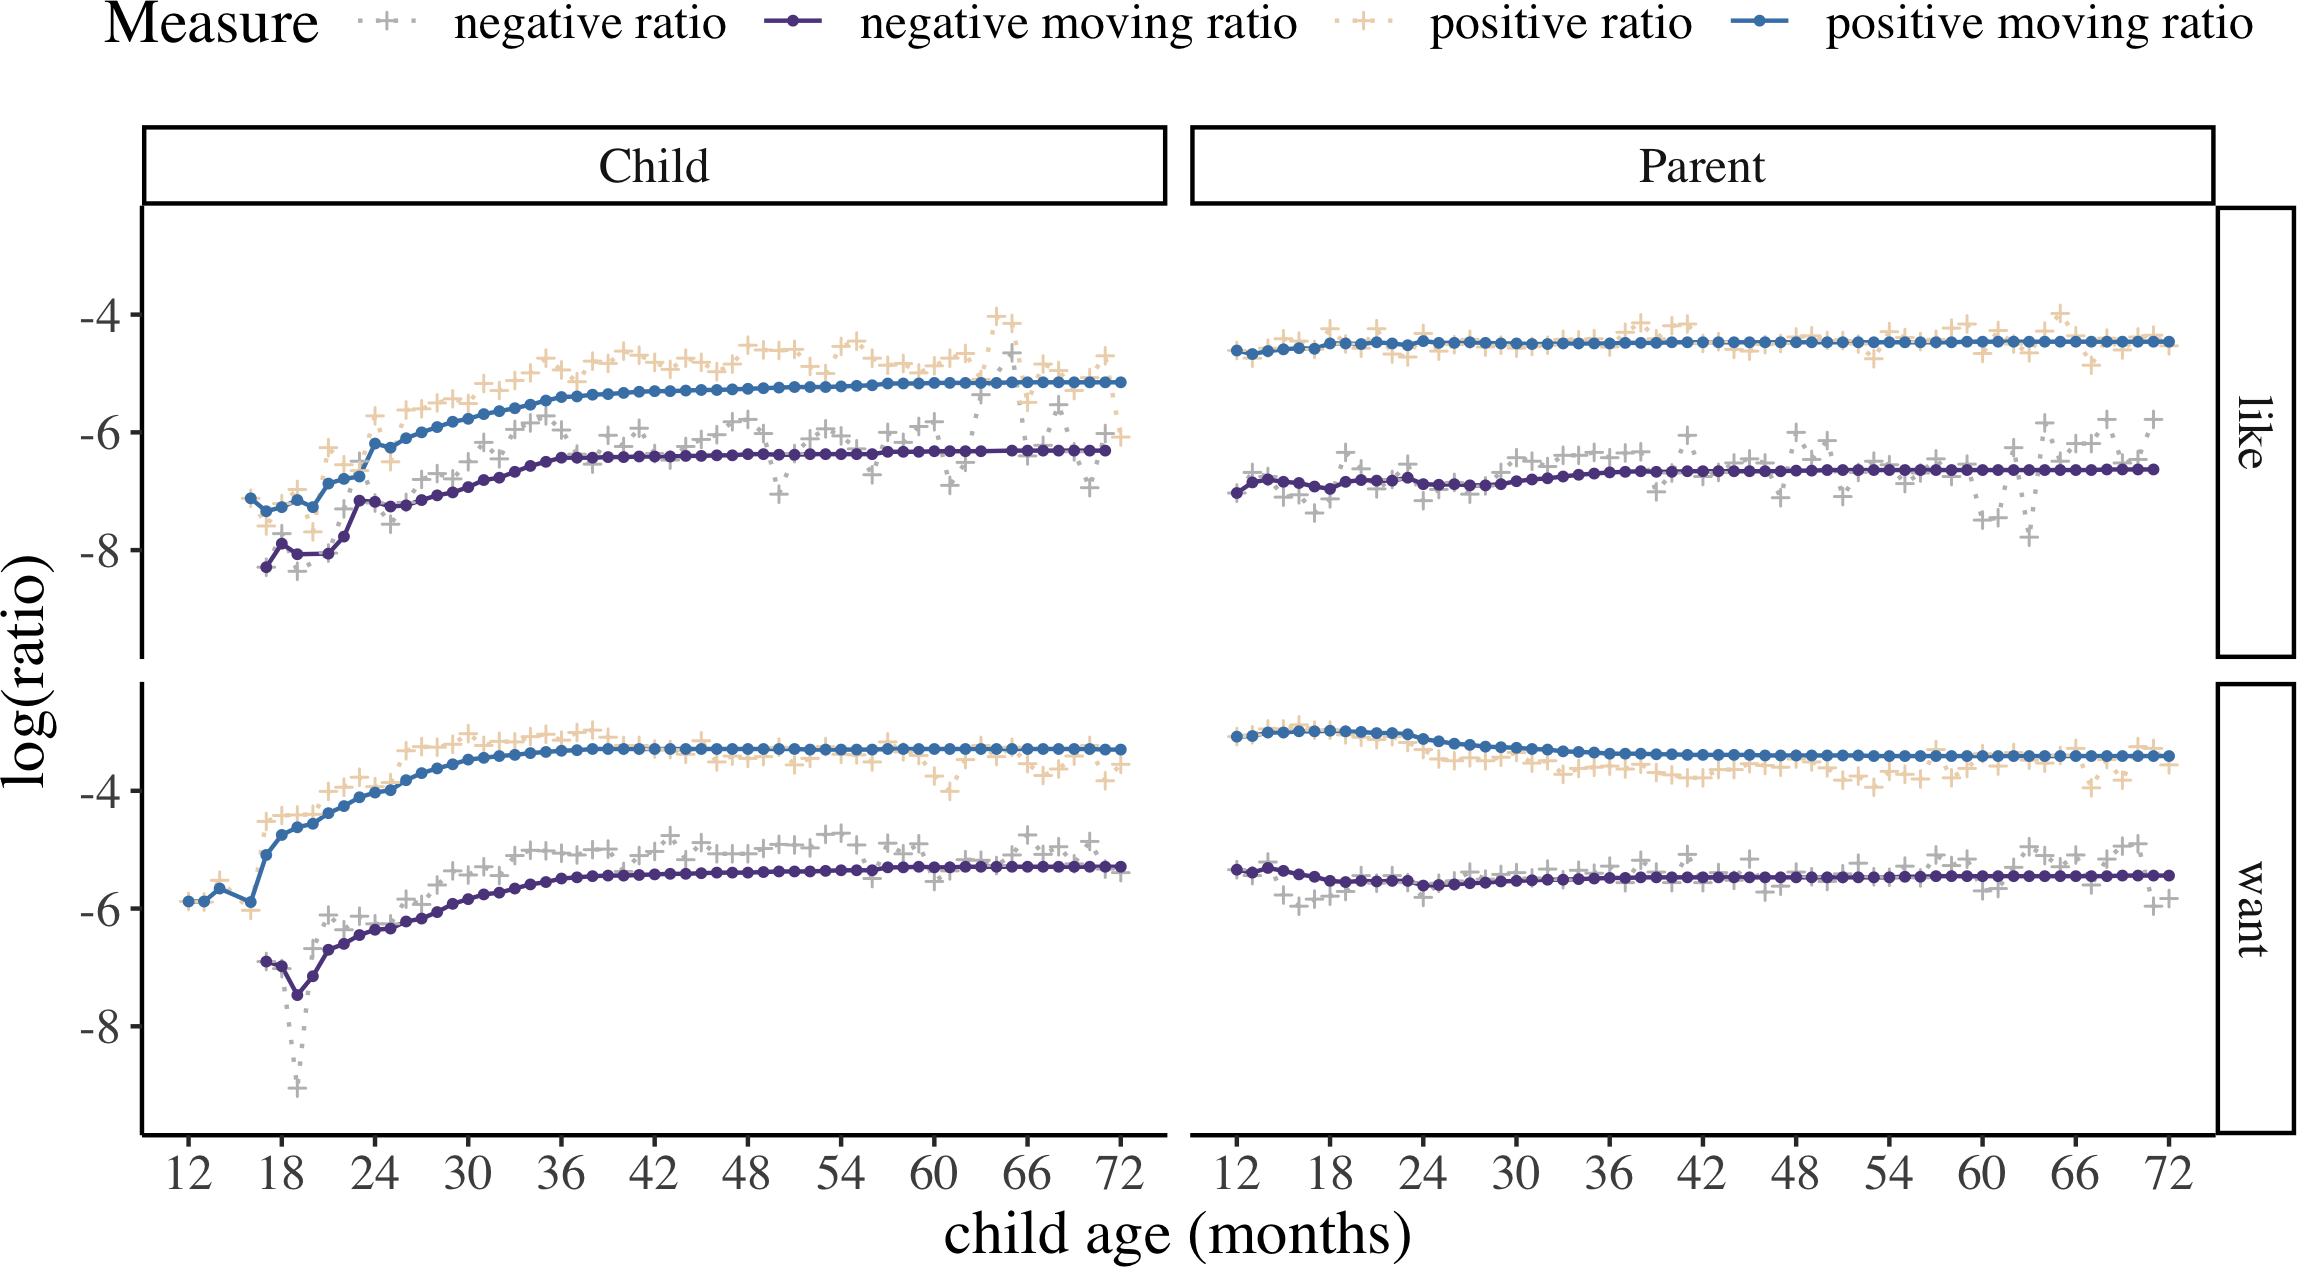
\includegraphics{results_files/figure-latex/emotion-1} 

}

\caption{Rejection}\label{fig:emotion}
\end{figure}

For both negative and positive:

Model: Production ratio \textasciitilde{} Age + MLU + Parent\_negative\_ratio + Parent\_Positive\_ratio + Parent\_negative\_MLU + Parent\_positive\_MLU

\begin{table}

\caption{\label{tab:unnamed-chunk-1}Estimating Production Ratio of Rejection in Child Speech, when head verb is like}
\centering
\begin{tabular}[t]{l|r|r|r|l}
\hline
Predictor & B & SE & t & p\\
\hline
Intercept & -32.32 & 5.830 & -5.54 & <0.001\\
\hline
Age & 0.01 & 0.002 & 4.52 & <0.001\\
\hline
MLU & -0.43 & 0.113 & -3.82 & <0.001\\
\hline
log(Parent\_negative\_ratio) & 3.70 & 0.405 & 9.13 & <0.001\\
\hline
log(Parent\_positive\_ratio) & -10.38 & 1.166 & -8.91 & <0.001\\
\hline
Parent\_negative\_MLU & -0.88 & 0.221 & -4.00 & <0.001\\
\hline
Parent\_positive\_MLU & 1.74 & 0.129 & 13.52 & <0.001\\
\hline
\end{tabular}
\end{table}

\begin{table}

\caption{\label{tab:unnamed-chunk-1}Estimating Production Ratio of Positive Counterparts for Rejection in Child Speech, when head verb is like}
\centering
\begin{tabular}[t]{l|r|r|r|l}
\hline
Predictor & B & SE & t & p\\
\hline
Intercept & -61.28 & 6.339 & -9.67 & <0.001\\
\hline
Age & 0.00 & 0.003 & -0.10 & 0.922\\
\hline
MLU & 0.77 & 0.107 & 7.24 & <0.001\\
\hline
log(Parent\_negative\_ratio) & 0.17 & 0.447 & 0.38 & 0.706\\
\hline
log(Parent\_positive\_ratio) & -10.81 & 1.221 & -8.86 & <0.001\\
\hline
Parent\_negative\_MLU & -0.92 & 0.239 & -3.86 & <0.001\\
\hline
Parent\_positive\_MLU & 1.56 & 0.132 & 11.82 & <0.001\\
\hline
\end{tabular}
\end{table}

\clearpage

\begin{table}

\caption{\label{tab:unnamed-chunk-2}Estimating Production Ratio of Rejection in Child Speech, when head verb is want}
\centering
\begin{tabular}[t]{l|r|r|r|l}
\hline
Predictor & B & SE & t & p\\
\hline
Intercept & 16.41 & 5.877 & 2.79 & 0.007\\
\hline
Age & 0.00 & 0.004 & -0.70 & 0.488\\
\hline
MLU & -0.09 & 0.051 & -1.70 & 0.095\\
\hline
log(Parent\_negative\_ratio) & 4.14 & 0.770 & 5.38 & <0.001\\
\hline
log(Parent\_positive\_ratio) & 1.85 & 1.139 & 1.62 & 0.111\\
\hline
Parent\_negative\_MLU & -1.69 & 0.400 & -4.22 & <0.001\\
\hline
Parent\_positive\_MLU & 3.06 & 0.563 & 5.44 & <0.001\\
\hline
\end{tabular}
\end{table}

\begin{table}

\caption{\label{tab:unnamed-chunk-2}Estimating Production Ratio of Positive Counterparts for Rejection in Child Speech, when head verb is want}
\centering
\begin{tabular}[t]{l|r|r|r|l}
\hline
Predictor & B & SE & t & p\\
\hline
Intercept & -19.36 & 6.372 & -3.04 & 0.004\\
\hline
Age & -0.01 & 0.004 & -3.53 & <0.001\\
\hline
MLU & -0.04 & 0.022 & -1.59 & 0.117\\
\hline
log(Parent\_negative\_ratio) & -0.39 & 0.772 & -0.50 & 0.617\\
\hline
log(Parent\_positive\_ratio) & 0.78 & 1.122 & 0.69 & 0.492\\
\hline
Parent\_negative\_MLU & -0.07 & 0.543 & -0.13 & 0.897\\
\hline
Parent\_positive\_MLU & 2.34 & 0.564 & 4.15 & <0.001\\
\hline
\end{tabular}
\end{table}

\clearpage

\hypertarget{non-existence}{%
\subsubsection{Non-existence}\label{non-existence}}

\begin{figure}[H]

{\centering 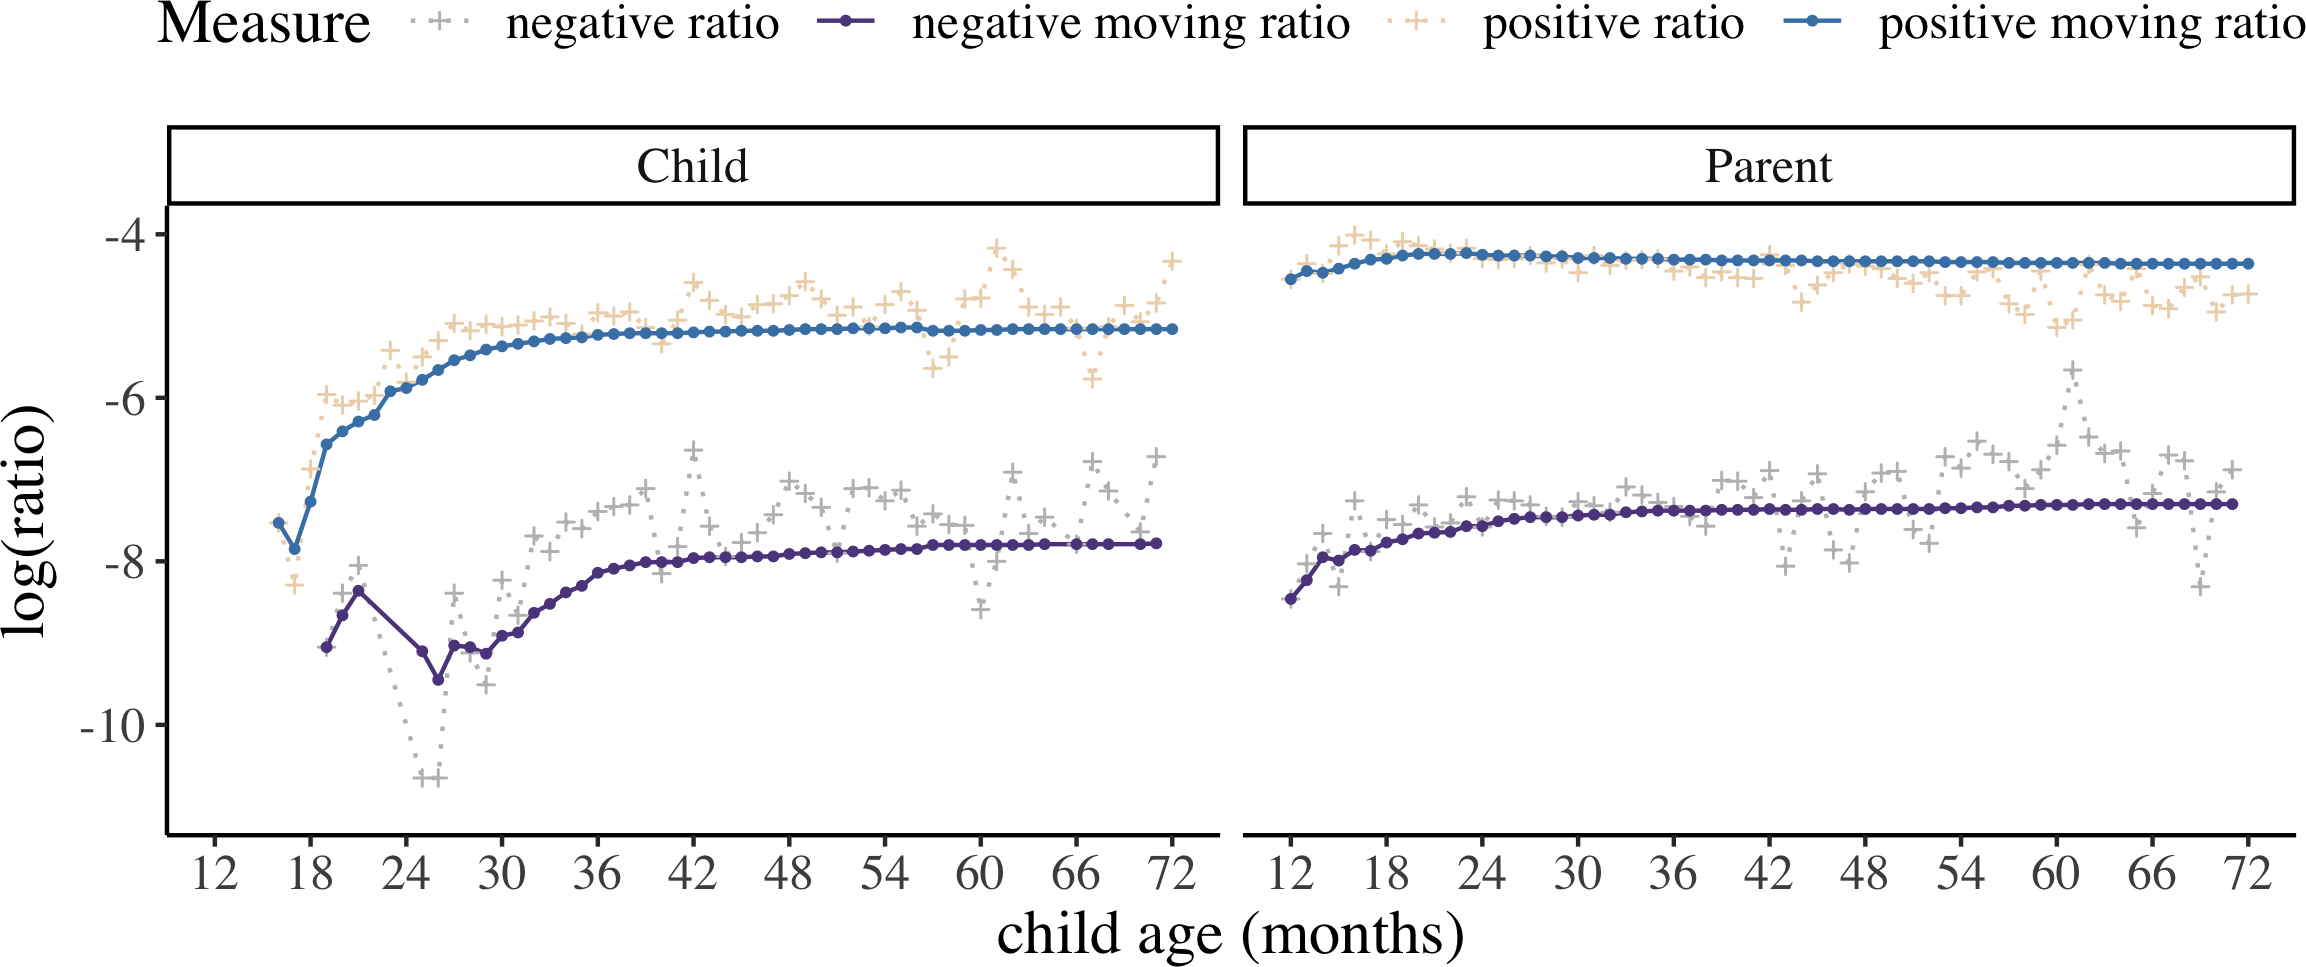
\includegraphics{results_files/figure-latex/existence-1} 

}

\caption{Non-existence}\label{fig:existence}
\end{figure}

\clearpage

\begin{table}

\caption{\label{tab:unnamed-chunk-3}Estimating Production Ratio of Non-existence in Child Speech}
\centering
\begin{tabular}[t]{l|r|r|r|l}
\hline
Predictor & B & SE & t & p\\
\hline
Intercept & -119.61 & 37.869 & -3.16 & 0.003\\
\hline
Age & -0.02 & 0.009 & -1.75 & 0.088\\
\hline
MLU & 0.18 & 0.283 & 0.62 & 0.538\\
\hline
log(Parent\_negative\_ratio) & 1.82 & 2.796 & 0.65 & 0.518\\
\hline
log(Parent\_positive\_ratio) & -31.65 & 10.579 & -2.99 & 0.005\\
\hline
Parent\_negative\_MLU & -1.39 & 0.493 & -2.82 & 0.007\\
\hline
Parent\_positive\_MLU & -0.09 & 1.176 & -0.08 & 0.940\\
\hline
\end{tabular}
\end{table}

\begin{table}

\caption{\label{tab:unnamed-chunk-3}Estimating Production Ratio of Positive Counterparts for Non-existence in Child Speech}
\centering
\begin{tabular}[t]{l|r|r|r|l}
\hline
Predictor & B & SE & t & p\\
\hline
Intercept & 35.29 & 5.571 & 6.33 & <0.001\\
\hline
Age & -0.01 & 0.003 & -2.86 & 0.006\\
\hline
MLU & 0.01 & 0.136 & 0.06 & 0.954\\
\hline
log(Parent\_negative\_ratio) & 4.02 & 0.620 & 6.49 & <0.001\\
\hline
log(Parent\_positive\_ratio) & 3.41 & 1.276 & 2.67 & 0.010\\
\hline
Parent\_negative\_MLU & -0.05 & 0.139 & -0.36 & 0.718\\
\hline
Parent\_positive\_MLU & 0.60 & 0.275 & 2.19 & 0.033\\
\hline
\end{tabular}
\end{table}

\clearpage

\hypertarget{prohibition}{%
\subsubsection{Prohibition}\label{prohibition}}

\begin{figure}[H]

{\centering 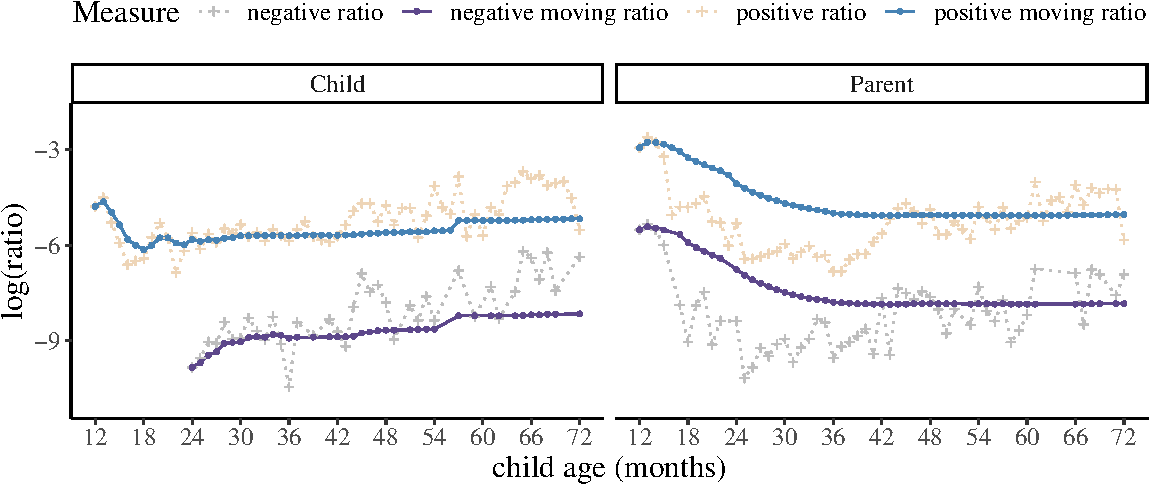
\includegraphics{results_files/figure-latex/prohibition-1} 

}

\caption{Prohibition}\label{fig:prohibition}
\end{figure}

\clearpage

\begin{table}

\caption{\label{tab:unnamed-chunk-4}Estimating Production Ratio of Prohibition in Child Speech}
\centering
\begin{tabular}[t]{l|r|r|r|l}
\hline
Predictor & B & SE & t & p\\
\hline
Intercept & -31.66 & 6.067 & -5.22 & <0.001\\
\hline
Age & 0.01 & 0.005 & 2.62 & 0.014\\
\hline
MLU & -0.15 & 0.134 & -1.13 & 0.270\\
\hline
log(Parent\_negative\_ratio) & -5.49 & 1.340 & -4.10 & <0.001\\
\hline
log(Parent\_positive\_ratio) & 5.31 & 1.509 & 3.52 & 0.002\\
\hline
Parent\_negative\_MLU & -1.25 & 0.709 & -1.76 & 0.089\\
\hline
Parent\_positive\_MLU & 2.73 & 0.821 & 3.32 & 0.003\\
\hline
\end{tabular}
\end{table}

\begin{table}

\caption{\label{tab:unnamed-chunk-4}Estimating Production Ratio of Positive Counterparts for Prohibition in Child Speech}
\centering
\begin{tabular}[t]{l|r|r|r|l}
\hline
Predictor & B & SE & t & p\\
\hline
Intercept & -7.76 & 10.108 & -0.77 & 0.447\\
\hline
Age & 0.00 & 0.010 & -0.05 & 0.957\\
\hline
MLU & 0.47 & 0.187 & 2.52 & 0.015\\
\hline
log(Parent\_negative\_ratio) & 0.98 & 1.546 & 0.63 & 0.530\\
\hline
log(Parent\_positive\_ratio) & -0.10 & 1.663 & -0.06 & 0.953\\
\hline
Parent\_negative\_MLU & 0.31 & 1.369 & 0.23 & 0.822\\
\hline
Parent\_positive\_MLU & 1.04 & 1.492 & 0.70 & 0.489\\
\hline
\end{tabular}
\end{table}

\clearpage

\hypertarget{inability}{%
\subsubsection{Inability}\label{inability}}

\begin{figure}[H]

{\centering 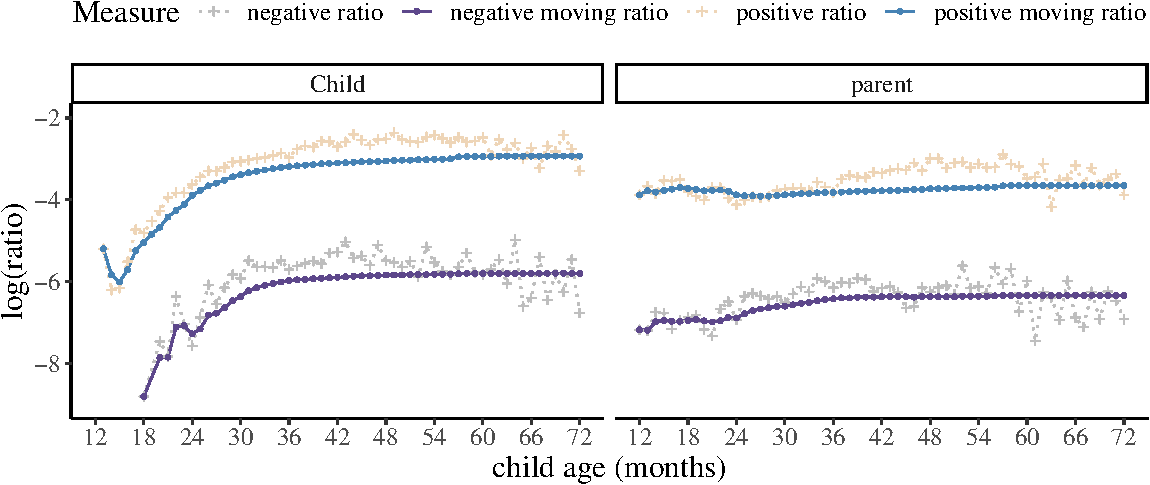
\includegraphics{results_files/figure-latex/inability-1} 

}

\caption{Inability}\label{fig:inability}
\end{figure}

\begin{table}

\caption{\label{tab:unnamed-chunk-5}Estimating Production Ratio of Inability in Child Speech}
\centering
\begin{tabular}[t]{l|r|r|r|l}
\hline
Predictor & B & SE & t & p\\
\hline
Intercept & 7.14 & 3.359 & 2.12 & 0.039\\
\hline
Age & 0.00 & 0.006 & 0.05 & 0.959\\
\hline
MLU & 1.04 & 0.117 & 8.85 & <0.001\\
\hline
log(Parent\_negative\_ratio) & 2.29 & 0.194 & 11.80 & <0.001\\
\hline
log(Parent\_positive\_ratio) & -0.59 & 0.464 & -1.28 & 0.208\\
\hline
Parent\_negative\_MLU & -0.08 & 0.290 & -0.27 & 0.789\\
\hline
Parent\_positive\_MLU & -0.75 & 0.390 & -1.93 & 0.060\\
\hline
\end{tabular}
\end{table}

\begin{table}

\caption{\label{tab:unnamed-chunk-5}Estimating Production Ratio of Positive Counterparts for Inability in Child Speech}
\centering
\begin{tabular}[t]{l|r|r|r|l}
\hline
Predictor & B & SE & t & p\\
\hline
Intercept & 1.35 & 4.518 & 0.30 & 0.766\\
\hline
Age & 0.02 & 0.005 & 3.80 & <0.001\\
\hline
MLU & -0.21 & 0.049 & -4.25 & <0.001\\
\hline
log(Parent\_negative\_ratio) & 2.14 & 0.268 & 7.98 & <0.001\\
\hline
log(Parent\_positive\_ratio) & -2.73 & 0.529 & -5.16 & <0.001\\
\hline
Parent\_negative\_MLU & -0.69 & 0.242 & -2.86 & 0.006\\
\hline
Parent\_positive\_MLU & 0.61 & 0.135 & 4.52 & <0.001\\
\hline
\end{tabular}
\end{table}

\clearpage

\hypertarget{labeling}{%
\subsubsection{Labeling}\label{labeling}}

\begin{figure}[H]

{\centering 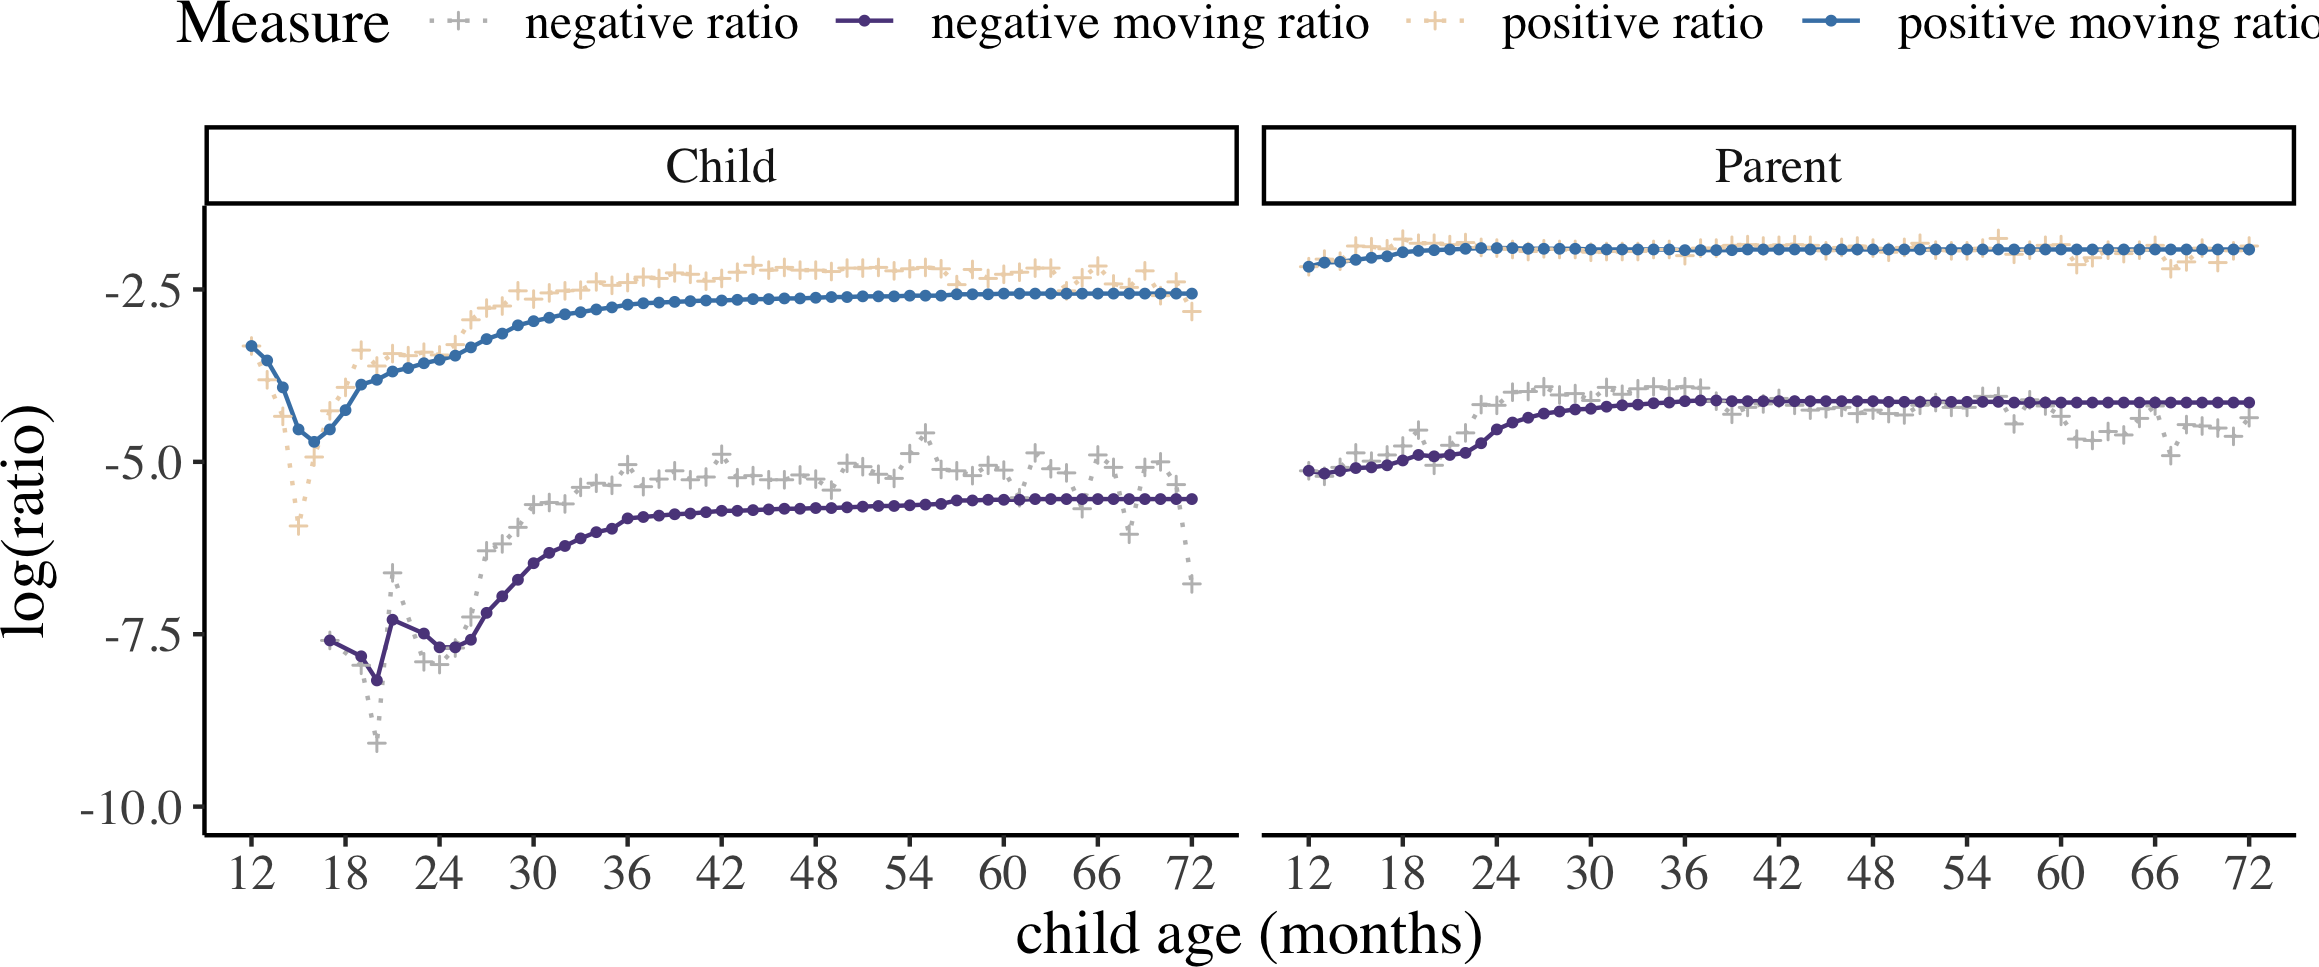
\includegraphics{results_files/figure-latex/learning-1} 

}

\caption{Language learning via labeling}\label{fig:learning}
\end{figure}

\clearpage

\begin{table}

\caption{\label{tab:unnamed-chunk-6}Estimating Production Ratio of Learning in Child Speech}
\centering
\begin{tabular}[t]{l|r|r|r|l}
\hline
Predictor & B & SE & t & p\\
\hline
Intercept & -43.58 & 10.055 & -4.33 & <0.001\\
\hline
Age & -0.01 & 0.008 & -0.93 & 0.359\\
\hline
MLU & 0.98 & 0.175 & 5.61 & <0.001\\
\hline
log(Parent\_negative\_ratio) & 2.82 & 0.768 & 3.67 & <0.001\\
\hline
log(Parent\_positive\_ratio) & -21.68 & 3.086 & -7.03 & <0.001\\
\hline
Parent\_negative\_MLU & -0.35 & 0.771 & -0.46 & 0.648\\
\hline
Parent\_positive\_MLU & 0.74 & 0.824 & 0.89 & 0.377\\
\hline
\end{tabular}
\end{table}

\begin{table}

\caption{\label{tab:unnamed-chunk-6}Estimating Production Ratio of Positive Counterparts for Learning in Child Speech}
\centering
\begin{tabular}[t]{l|r|r|r|l}
\hline
Predictor & B & SE & t & p\\
\hline
Intercept & 7.47 & 5.347 & 1.40 & 0.168\\
\hline
Age & -0.01 & 0.005 & -2.00 & 0.051\\
\hline
MLU & 1.48 & 0.217 & 6.78 & <0.001\\
\hline
log(Parent\_negative\_ratio) & 1.12 & 0.275 & 4.08 & <0.001\\
\hline
log(Parent\_positive\_ratio) & 3.14 & 1.170 & 2.68 & 0.010\\
\hline
Parent\_negative\_MLU & -0.11 & 0.439 & -0.24 & 0.812\\
\hline
Parent\_positive\_MLU & -0.86 & 0.447 & -1.92 & 0.060\\
\hline
\end{tabular}
\end{table}

\clearpage

\hypertarget{epistemic-negation}{%
\subsubsection{Epistemic Negation}\label{epistemic-negation}}

\begin{figure}[H]

{\centering 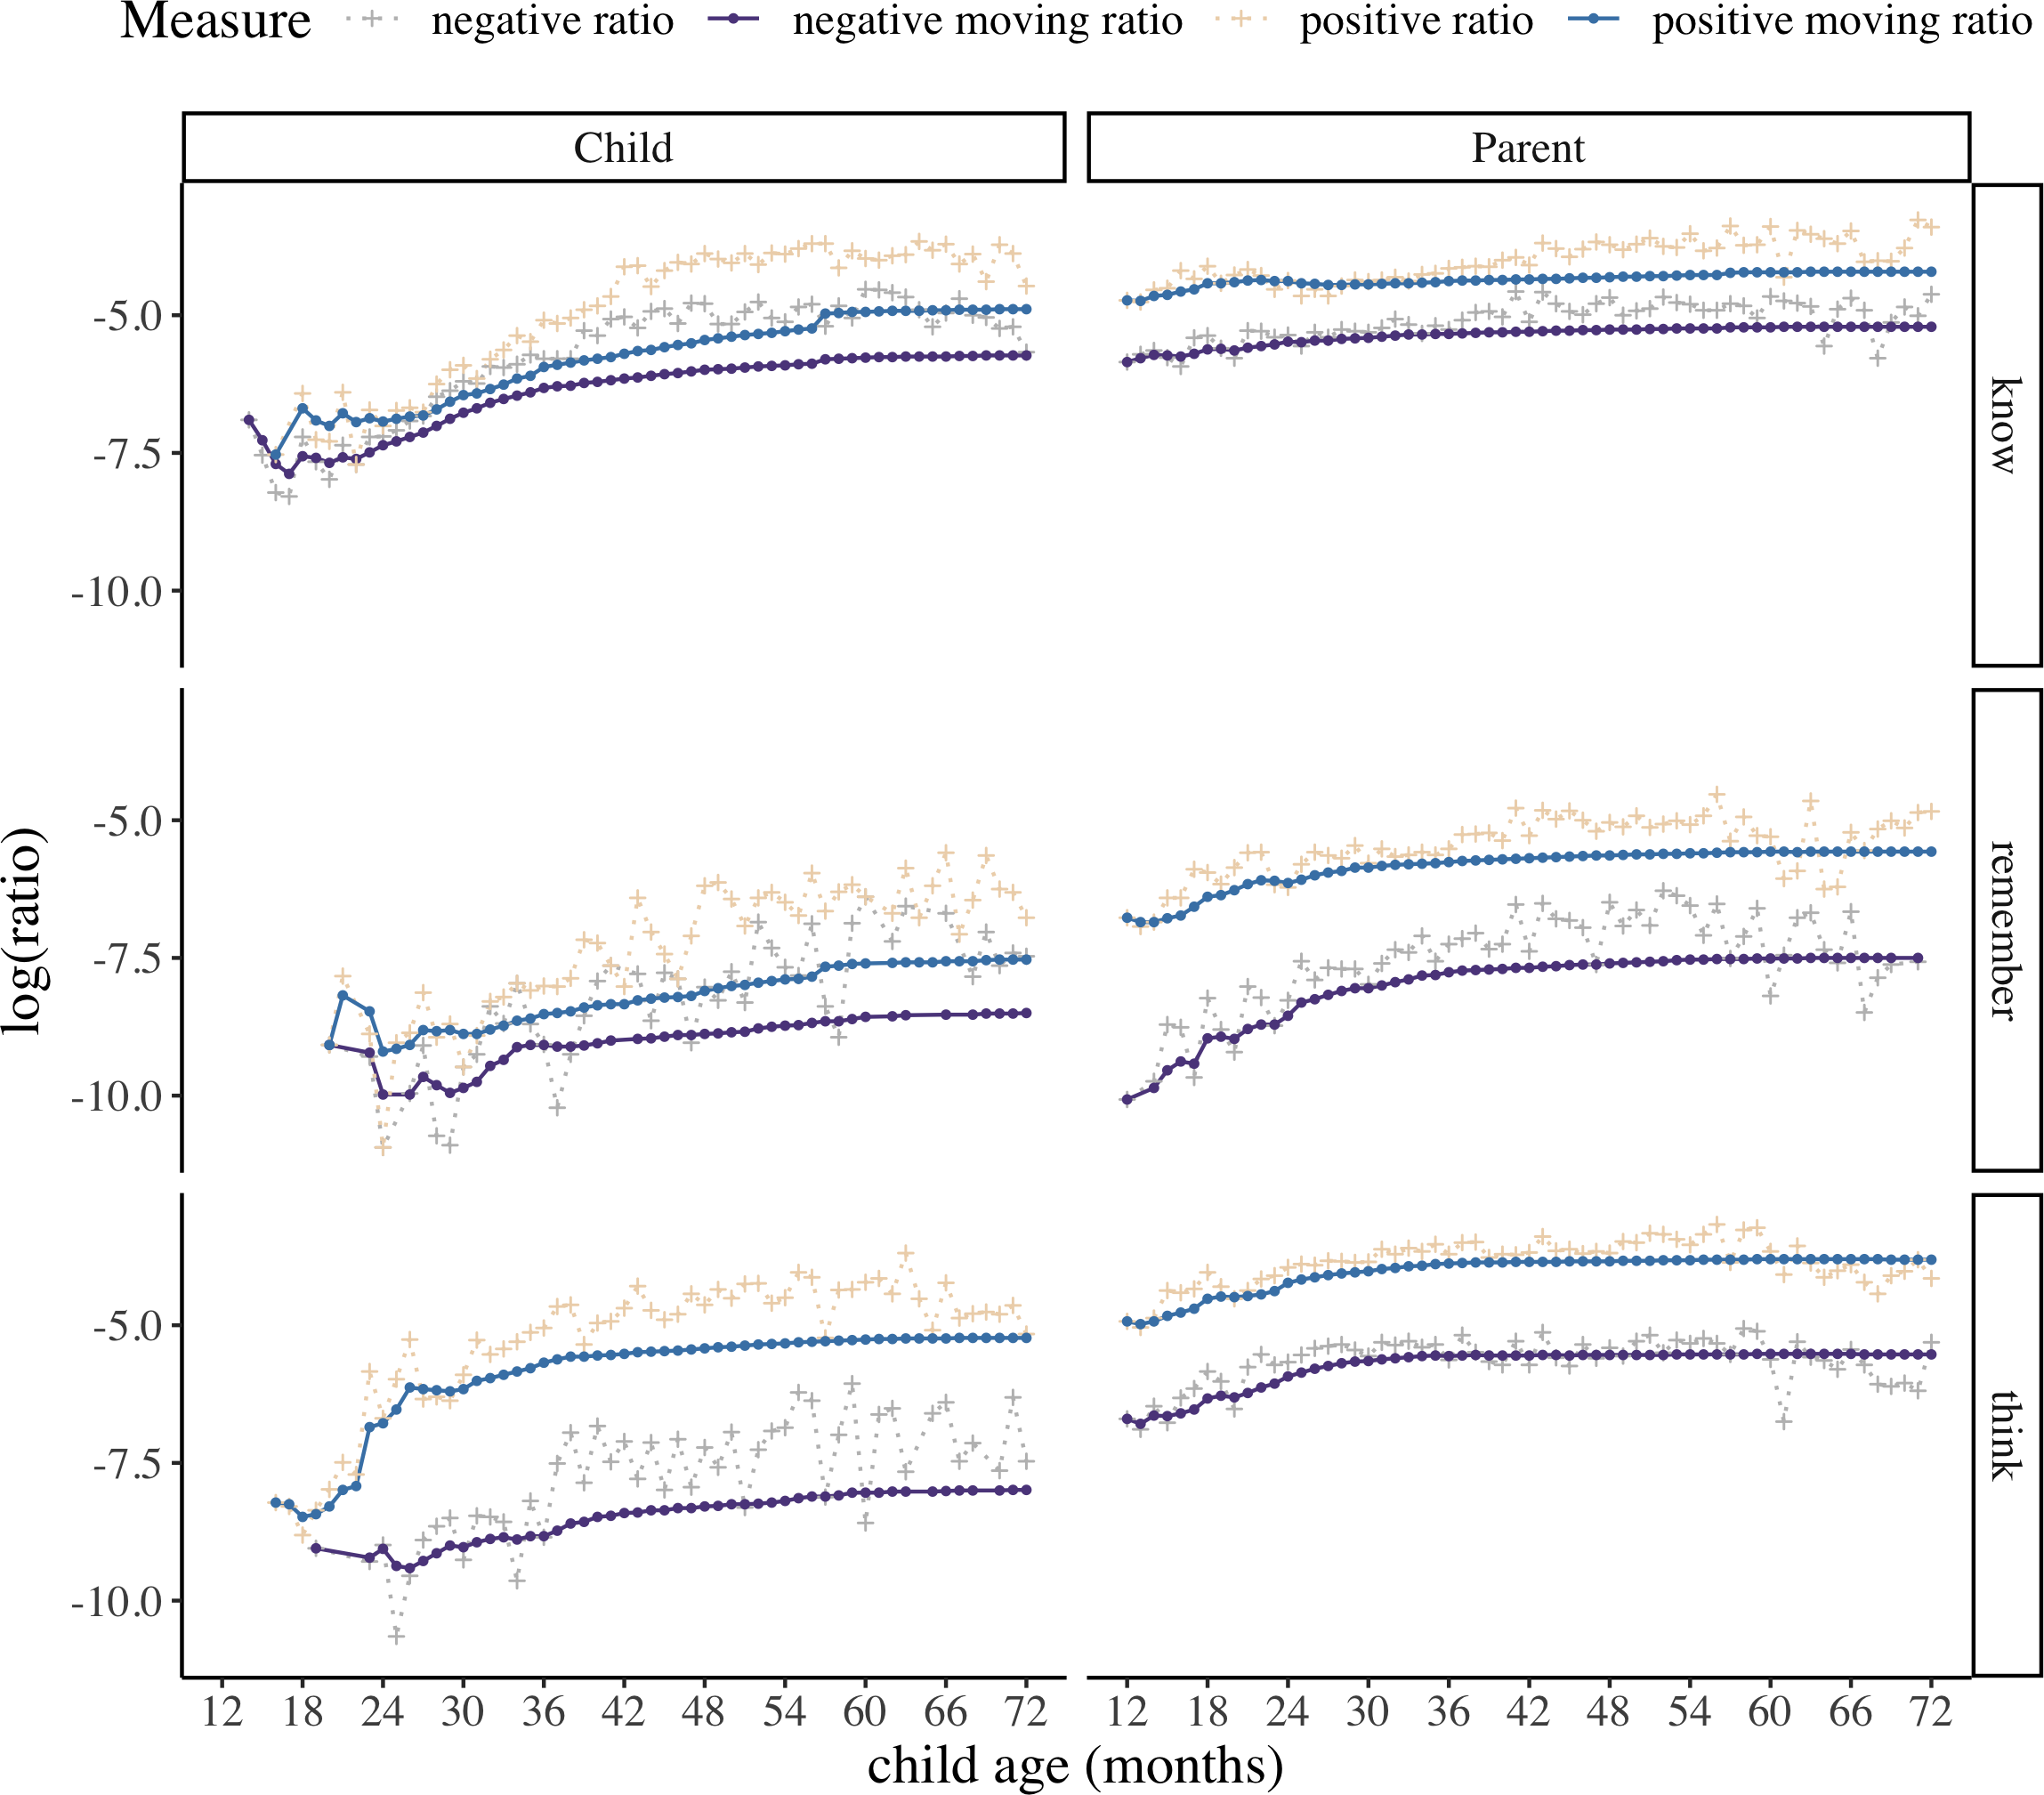
\includegraphics{results_files/figure-latex/epistemic-1} 

}

\caption{Epistemic negation}\label{fig:epistemic}
\end{figure}

\clearpage

\begin{table}

\caption{\label{tab:unnamed-chunk-7}Estimating Production Ratio of Epistemic Negation in Child Speech, when head verb is know}
\centering
\begin{tabular}[t]{l|r|r|r|l}
\hline
Predictor & B & SE & t & p\\
\hline
Intercept & 19.99 & 2.065 & 9.68 & <0.001\\
\hline
Age & 0.00 & 0.002 & 0.48 & 0.632\\
\hline
MLU & 0.14 & 0.030 & 4.55 & <0.001\\
\hline
log(Parent\_negative\_ratio) & 4.00 & 0.384 & 10.42 & <0.001\\
\hline
log(Parent\_positive\_ratio) & 0.40 & 0.341 & 1.16 & 0.249\\
\hline
Parent\_negative\_MLU & 0.00 & 0.144 & 0.03 & 0.973\\
\hline
Parent\_positive\_MLU & -0.47 & 0.103 & -4.57 & <0.001\\
\hline
\end{tabular}
\end{table}

\begin{table}

\caption{\label{tab:unnamed-chunk-7}Estimating Production Ratio of Positive Counterparts for Epistemic Negation in Child Speech, when head verb is know}
\centering
\begin{tabular}[t]{l|r|r|r|l}
\hline
Predictor & B & SE & t & p\\
\hline
Intercept & 17.04 & 3.045 & 5.60 & <0.001\\
\hline
Age & 0.01 & 0.002 & 4.11 & <0.001\\
\hline
MLU & 0.28 & 0.040 & 7.12 & <0.001\\
\hline
log(Parent\_negative\_ratio) & 2.43 & 0.514 & 4.72 & <0.001\\
\hline
log(Parent\_positive\_ratio) & 2.00 & 0.406 & 4.94 & <0.001\\
\hline
Parent\_negative\_MLU & 0.17 & 0.187 & 0.89 & 0.380\\
\hline
Parent\_positive\_MLU & -0.54 & 0.146 & -3.73 & <0.001\\
\hline
\end{tabular}
\end{table}

\clearpage

\begin{table}

\caption{\label{tab:unnamed-chunk-8}Estimating Production Ratio of Epistemic Negation in Child Speech, when head verb is remember}
\centering
\begin{tabular}[t]{l|r|r|r|l}
\hline
Predictor & B & SE & t & p\\
\hline
Intercept & 48.04 & 9.766 & 4.92 & <0.001\\
\hline
Age & 0.03 & 0.005 & 5.88 & <0.001\\
\hline
MLU & 0.08 & 0.086 & 0.92 & 0.364\\
\hline
log(Parent\_negative\_ratio) & -4.60 & 1.460 & -3.15 & 0.003\\
\hline
log(Parent\_positive\_ratio) & 11.97 & 2.279 & 5.25 & <0.001\\
\hline
Parent\_negative\_MLU & -1.28 & 0.340 & -3.77 & <0.001\\
\hline
Parent\_positive\_MLU & -1.88 & 0.421 & -4.45 & <0.001\\
\hline
\end{tabular}
\end{table}

\begin{table}

\caption{\label{tab:unnamed-chunk-8}Estimating Production Ratio of Positive Counterparts for Epistemic Negation in Child Speech, when head verb is remember}
\centering
\begin{tabular}[t]{l|r|r|r|l}
\hline
Predictor & B & SE & t & p\\
\hline
Intercept & 13.74 & 5.327 & 2.58 & 0.014\\
\hline
Age & 0.02 & 0.004 & 4.25 & <0.001\\
\hline
MLU & 0.23 & 0.053 & 4.40 & <0.001\\
\hline
log(Parent\_negative\_ratio) & -1.07 & 0.646 & -1.65 & 0.106\\
\hline
log(Parent\_positive\_ratio) & 4.49 & 0.862 & 5.21 & <0.001\\
\hline
Parent\_negative\_MLU & 0.03 & 0.152 & 0.21 & 0.833\\
\hline
Parent\_positive\_MLU & -0.83 & 0.231 & -3.57 & <0.001\\
\hline
\end{tabular}
\end{table}

\clearpage

\begin{table}

\caption{\label{tab:unnamed-chunk-9}Estimating Production Ratio of Epistemic Negation in Child Speech, when head verb is think}
\centering
\begin{tabular}[t]{l|r|r|r|l}
\hline
Predictor & B & SE & t & p\\
\hline
Intercept & -9.65 & 4.076 & -2.37 & 0.023\\
\hline
Age & 0.02 & 0.004 & 4.77 & <0.001\\
\hline
MLU & 0.07 & 0.065 & 1.05 & 0.299\\
\hline
log(Parent\_negative\_ratio) & -2.64 & 1.021 & -2.58 & 0.013\\
\hline
log(Parent\_positive\_ratio) & 3.26 & 1.324 & 2.46 & 0.018\\
\hline
Parent\_negative\_MLU & 0.97 & 0.839 & 1.15 & 0.255\\
\hline
Parent\_positive\_MLU & -1.28 & 0.802 & -1.60 & 0.118\\
\hline
\end{tabular}
\end{table}

\begin{table}

\caption{\label{tab:unnamed-chunk-9}Estimating Production Ratio of Positive Counterparts for Epistemic Negation in Child Speech, when head verb is think}
\centering
\begin{tabular}[t]{l|r|r|r|l}
\hline
Predictor & B & SE & t & p\\
\hline
Intercept & 26.43 & 2.182 & 12.11 & <0.001\\
\hline
Age & 0.01 & 0.002 & 4.66 & <0.001\\
\hline
MLU & 0.55 & 0.049 & 11.28 & <0.001\\
\hline
log(Parent\_negative\_ratio) & 0.10 & 0.501 & 0.20 & 0.843\\
\hline
log(Parent\_positive\_ratio) & 2.26 & 0.540 & 4.18 & <0.001\\
\hline
Parent\_negative\_MLU & -1.93 & 0.277 & -6.95 & <0.001\\
\hline
Parent\_positive\_MLU & -0.82 & 0.071 & -11.58 & <0.001\\
\hline
\end{tabular}
\end{table}

\clearpage

\hypertarget{possession}{%
\subsubsection{Possession}\label{possession}}

\begin{figure}[H]

{\centering 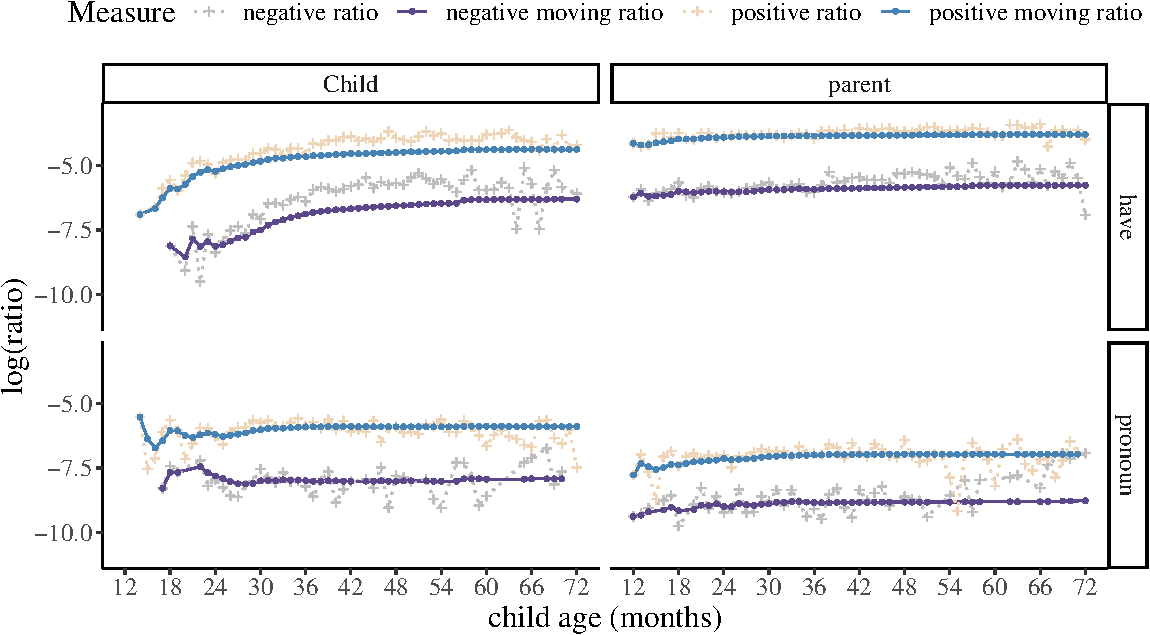
\includegraphics{results_files/figure-latex/possession-1} 

}

\caption{Possession}\label{fig:possession}
\end{figure}

\clearpage

\begin{table}

\caption{\label{tab:unnamed-chunk-10}Estimating Production Ratio of Posession in Child Speech, when head verb is have}
\centering
\begin{tabular}[t]{l|r|r|r|l}
\hline
Predictor & B & SE & t & p\\
\hline
Intercept & 34.85 & 16.952 & 2.06 & 0.046\\
\hline
Age & 0.00 & 0.005 & 0.81 & 0.420\\
\hline
MLU & -0.01 & 0.061 & -0.09 & 0.928\\
\hline
log(Parent\_negative\_ratio) & 5.67 & 1.270 & 4.46 & <0.001\\
\hline
log(Parent\_positive\_ratio) & -1.07 & 4.987 & -0.21 & 0.831\\
\hline
Parent\_negative\_MLU & -2.14 & 0.285 & -7.52 & <0.001\\
\hline
Parent\_positive\_MLU & 1.02 & 0.439 & 2.32 & 0.025\\
\hline
\end{tabular}
\end{table}

\begin{table}

\caption{\label{tab:unnamed-chunk-10}Estimating Production Ratio of Positive Counterparts for Posession in Child Speech, when syntactic head is pronoun}
\centering
\begin{tabular}[t]{l|r|r|r|l}
\hline
Predictor & B & SE & t & p\\
\hline
Intercept & 43.40 & 3.955 & 10.97 & <0.001\\
\hline
Age & 0.00 & 0.002 & -0.01 & 0.988\\
\hline
MLU & 0.11 & 0.045 & 2.52 & 0.015\\
\hline
log(Parent\_negative\_ratio) & -0.82 & 0.439 & -1.86 & 0.068\\
\hline
log(Parent\_positive\_ratio) & 11.09 & 0.772 & 14.36 & <0.001\\
\hline
Parent\_negative\_MLU & -0.98 & 0.115 & -8.54 & <0.001\\
\hline
Parent\_positive\_MLU & -0.15 & 0.096 & -1.53 & 0.132\\
\hline
\end{tabular}
\end{table}

\clearpage

\begin{table}

\caption{\label{tab:unnamed-chunk-11}Estimating Production Ratio of Positive Counterparts for Posession in Child Speech, when head verb is want}
\centering
\begin{tabular}[t]{l|r|r|r|l}
\hline
Predictor & B & SE & t & p\\
\hline
Intercept & -20.45 & 3.523 & -5.80 & <0.001\\
\hline
Age & 0.01 & 0.002 & 3.14 & 0.004\\
\hline
MLU & 0.20 & 0.100 & 2.01 & 0.054\\
\hline
log(Parent\_negative\_ratio) & -0.34 & 0.421 & -0.80 & 0.432\\
\hline
log(Parent\_positive\_ratio) & -2.15 & 0.616 & -3.49 & 0.002\\
\hline
Parent\_negative\_MLU & -1.51 & 0.162 & -9.31 & <0.001\\
\hline
Parent\_positive\_MLU & 0.36 & 0.168 & 2.17 & 0.038\\
\hline
\end{tabular}
\end{table}

\begin{table}

\caption{\label{tab:unnamed-chunk-11}Estimating Production Ratio of Positive Counterparts for Posession in Child Speech, when syntactic head is pronoun}
\centering
\begin{tabular}[t]{l|r|r|r|l}
\hline
Predictor & B & SE & t & p\\
\hline
Intercept & -23.32 & 8.974 & -2.60 & 0.013\\
\hline
Age & 0.00 & 0.003 & -0.83 & 0.410\\
\hline
MLU & 1.17 & 0.407 & 2.87 & 0.007\\
\hline
log(Parent\_negative\_ratio) & -1.36 & 0.611 & -2.23 & 0.032\\
\hline
log(Parent\_positive\_ratio) & -0.53 & 1.306 & -0.41 & 0.687\\
\hline
Parent\_negative\_MLU & -0.22 & 0.300 & -0.74 & 0.462\\
\hline
Parent\_positive\_MLU & -0.31 & 0.283 & -1.10 & 0.280\\
\hline
\end{tabular}
\end{table}

\begingroup
\setlength{\parindent}{-0.5in}
\setlength{\leftskip}{0.5in}

\endgroup

\hypertarget{refs}{}
\leavevmode\hypertarget{ref-bloom1970language}{}%
Bloom, L. M. (1970). \emph{Language development: Form and function in emerging grammars} (PhD thesis). Columbia University.

\leavevmode\hypertarget{ref-cameron2007part}{}%
Cameron-Faulkner, T., Lieven, E., \& Theakston, A. (2007). What part of no do children not understand? A usage-based account of multiword negation. \emph{Journal of Child Language}, \emph{34}(2), 251.

\leavevmode\hypertarget{ref-choi1988semantic}{}%
Choi, S. (1988). The semantic development of negation: A cross-linguistic longitudinal study. \emph{Journal of Child Language}, \emph{15}(3), 517--531.

\leavevmode\hypertarget{ref-clark2010adult}{}%
Clark, E. V. (2010). Adult offer, word-class, and child uptake in early lexical acquisition. \emph{First Language}, \emph{30}(3-4), 250--269.

\leavevmode\hypertarget{ref-darwin1872expression}{}%
Darwin, C. (1872). \emph{The expression of the emotions in man and animals}. John Murray.

\leavevmode\hypertarget{ref-demuth2006word}{}%
Demuth, K., Culbertson, J., \& Alter, J. (2006). Word-minimality, epenthesis and coda licensing in the early acquisition of English. \emph{Language and Speech}, \emph{49}(2), 137--173.

\leavevmode\hypertarget{ref-macwhinney2000childes}{}%
MacWhinney, B. (2000). \emph{The childes project: Tools for analyzing talk. Transcription format and programs} (Vol. 1). Psychology Press.

\leavevmode\hypertarget{ref-nordmeyer2018individual}{}%
Nordmeyer, A., \& Frank, M. C. (2018). Individual variation in children's early production of negation. In \emph{CogSci}.

\leavevmode\hypertarget{ref-pea1978}{}%
Pea, R. (1978). \emph{The development of negation in early child language} (PhD thesis). University of Oxford.

\leavevmode\hypertarget{ref-sagae2010morphosyntactic}{}%
Sagae, K., Davis, E., Lavie, A., MacWhinney, B., \& Wintner, S. (2010). Morphosyntactic annotation of childes transcripts. \emph{Journal of Child Language}, \emph{37}(3), 705--729.

\leavevmode\hypertarget{ref-de1979form}{}%
Villiers, P. A. de, \& Villiers, J. G. de. (1979). Form and function in the development of sentence negation. \emph{Papers and Reports on Child Language Development}, \emph{17}, 57--64.


\end{document}
